% Section 4.7 convergence figure; built by figures/build_convergence.py from
% figures/source_data/convergence_igd.csv (exported by
% .workbuddy/run_scripts/ExportConvergenceCSV.m).
\begin{figure*}[t]
  \centering
  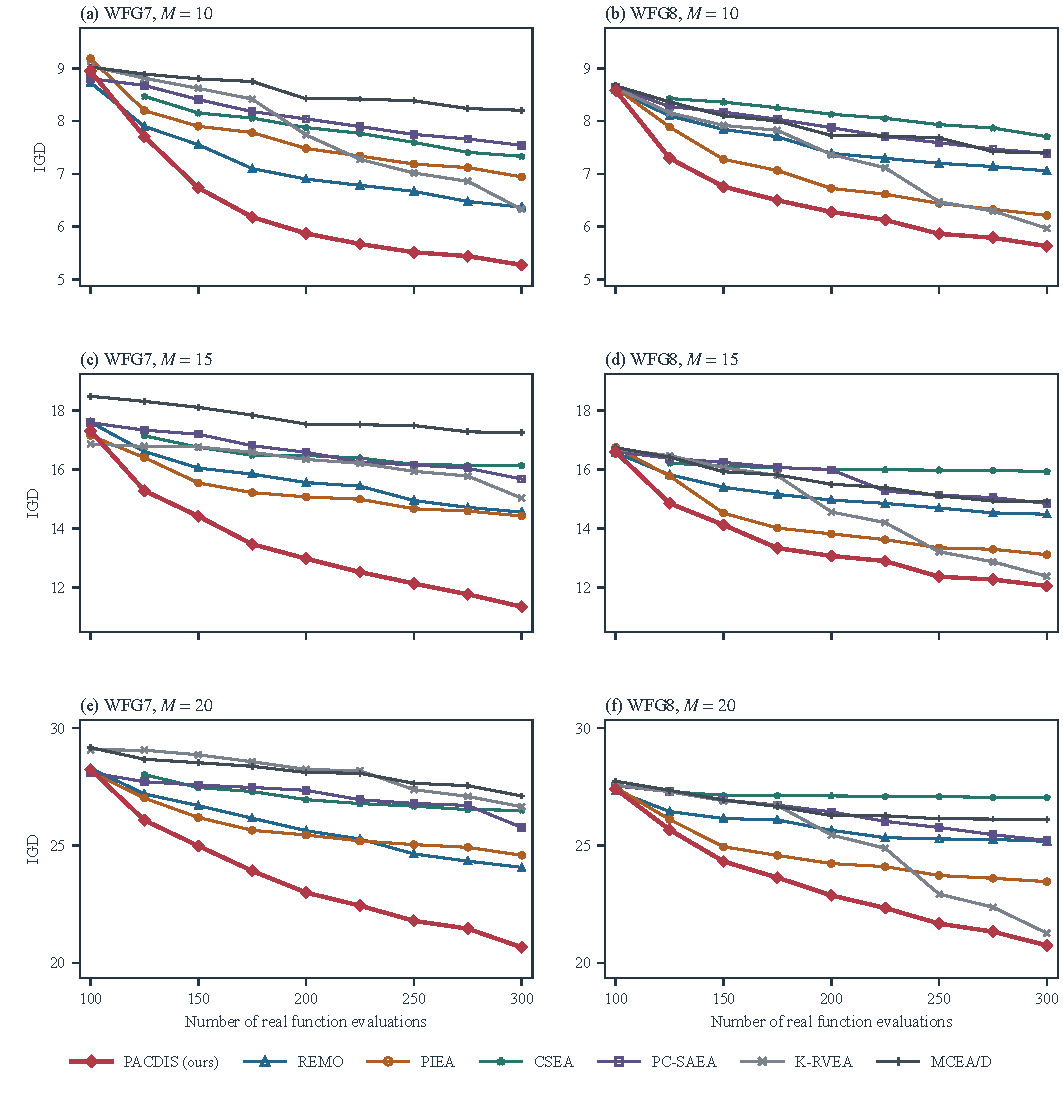
\includegraphics[width=0.98\textwidth]{figures/fig_convergence.pdf}
  \caption{Median IGD convergence of PACDIS and the six baseline algorithms
  on WFG7 and WFG8 at $M=10$, 15 and 20. Each curve summarizes 20
  independent runs (run identifiers 1--20) of the same experiment as the
  main comparison and starts at the algorithm's first recorded snapshot,
  because the initial design already consumes real evaluations. Traces are
  aligned on a unit-FE grid by holding the most recent recorded value,
  without extrapolation past the last snapshot, and one vertex is drawn
  every 25 evaluations. The IGD values are computed by the same
  implementation and reference sets as
  Tables~\ref{tab:exp:dtlz} and~\ref{tab:exp:wfg}.}
  \label{fig:exp:convergence}
\end{figure*}
